\documentclass{article} % ICLR 2027 conference paper
\usepackage{iclr2027_conference,times}
\input{math_commands.tex}
\usepackage{amsmath,amssymb,amsfonts}
\usepackage{graphicx}
\usepackage{booktabs}
\usepackage{multirow}
\usepackage{enumitem}
\usepackage{hyperref}
\usepackage{url}
\usepackage{xcolor}

\newcommand{\taustruct}{\tau_{\mathrm{struct}}}
\newcommand{\tautrap}{\tau_{\mathrm{trap}}}
\newcommand{\taureplay}{\tau_{\mathrm{replay}}}
\newcommand{\tauctx}{\tau_{\mathrm{context}}}
\newcommand{\taupxs}{\tau_{P\times S}}
\newcommand{\hfr}{\mathrm{HFR}}

\title{What Are Agent-Memory Gains Made Of?\\ Factorially Decomposing Replay, Structural Transfer,\\ and Surface Traps with Evaluator-Only Program Oracles}

\author{Anonymous}

\begin{document}
\maketitle

\begin{abstract}
Agent memory systems report consistent aggregate improvements from storing and reusing past episodes, but aggregate accuracy cannot tell \emph{what} the gain is made of: exact replay of seen episodes, reuse of a transferable procedure under surface change, or surface-matched exploitation of an incompatible program. We decompose these channels with a benchmark of latent-program task families in which program match ($P$) and surface similarity ($S$) are independently randomized per memory--target pair while family, program, and transformation labels remain evaluator-only. Across 7{,}680 fixed-injection rollouts of two frozen models and a pre-registered validity audit (strong leakage probes, difficulty equivalence, continuous-similarity sensitivity, oracle re-execution), we find: (i) aggregate gains are replay-dominated---in our 7B setting $72\%$ of the matched-content effect comes from the surface-matched leg---and the clean structural-transfer term changes sign with model scale ($\taustruct = +0.092$ [Holm-significant] for 7B vs.\ negative for 3B with a significant $P\times S$ interaction), revising the ``weaker models benefit more'' conclusion drawn from system-level aggregates; (ii) near-miss memories cause paired harmful flips (3B: $18.8\%$; 7B: $9.2\%$) concentrated in states where the vis-\'a-vis programs semantically diverge; and (iii) in a fresh 2-by-2 factorial separating representation \emph{form} from semantic \emph{coverage} (9216 rollouts on 32 held-out families), replay realization is governed by coverage completeness---preserving the decision and termination steps---not by representation form: even full transcripts realize replay materially (TOST rejects a $\pm3$pp equivalence), necessarily revising an earlier negative result we report. Method-comparison baselines (an architecture$\times$content transplant baseline, an embedding-based structural signal, and an LLM intent-mismatch judge) fail to recover these quantities in our harness. Deploying the coverage finding as a deterministic decision-aware compression policy beats naive top-truncation at exactly paired per-card token budgets on the pooled grid ($+14.5$pp replay realization at 7B, Holm-significant; at 3B there is no pooled evidence of benefit, point estimate $-8.4$pp, which we report with the same prominence) without degrading the primary harmful-flip guardrail at either scale (the secondary trap-shift bound is established only at 7B); a provenance-stratified sensitivity then shows the pooled 7B advantage is carried by oracle-reconstructed source episodes (direct interaction $+0.38$, CI excluding zero) and is not established on authentic model trajectories ($+4.1$pp, CI crossing zero), and we bound the deployment claim accordingly (12{,}800 rollouts). We release all generators, sealed-oracle evaluators, rollouts, and analysis code.
\end{abstract}

\section{Introduction}

Language agents increasingly improve at deployment time by reading from an external store of \emph{memories} distilled from past episodes---verbatim trajectories, distilled reflections, procedure cards, learned workflows \citep{shinn2023reflexion,zhao2024expel,wang2025awm,fang2025memp,mcma2026,reme2026}. Reported gains are usually computed as an \emph{aggregate} effect: task-level success with memory minus success without it. Behind a single such number, however, at least three radically different causal channels can coexist:

\begin{enumerate}[leftmargin=1.6em]
  \item \textbf{Exact or near-exact replay.} The current task reproduces something the memory literally described, so the gain is recall of an instance, not learning.
  \item \textbf{Structural (procedural) transfer.} A procedure genuinely crosses surface change---different entities, wording, domain vocabulary---because the memory encodes a reusable program.
  \item \textbf{Surface exploitation and surface traps.} Tasks whose surface cues match receive (mis)guidance; when the cues are similar but the required program is different, the memory can actively hurt---a harmful flip of a task the agent would otherwise solve.
\end{enumerate}

No aggregate metric distinguishes these channels, yet they carry opposite deployment meanings: replay justifies a cache, structural transfer justifies learning, traps justify admission control. Worse, the ``memory effect positive / weak models benefit more'' narratives \citep{feng2026transplants,procedmem2025,stitch2026camebench} are all stated at the aggregate level, and \citet{memdelta2026,bridge2026} have already warned that pipeline and counterfactual confounds can fabricate or erase the conclusions.

\textbf{Question.} \emph{Under identical model, budget, retriever, and prompt, what is the observed memory gain made of?} Precisely: how much of the improvement over no-memory, per memory--target pair, comes from (i) exact replay-like reuse, (ii) clean structural transfer under surface change, (iii) context/format overhead, and (iv) near-miss harm? And which of those components survives a pre-registered separation of representation \emph{form} from semantic \emph{coverage}?

\textbf{Answer.} We introduce \emph{CausalMemBench}, a generator of latent-program task families (four confirmation archetypes rendered into four business domains), a sealed oracle that holds the program-equivalence labels evaluator-only, and a $P\times S$ factorial design (Stage A) that independently randomizes latent program match $P\in\{0,1\}$ and surface similarity $S\in\{0,1\}$ for each memory--target pair. The cells read: A00 (unrelated control), A01 (surface trap / near-miss), A10 (clean structural transfer), A11 (replay-like reuse), plus no-memory (N) and sham-memory (Q) references. We run a 40-family mini-pilot with frozen Qwen2.5-3B/7B, a 200-token-budget-matched injection, and family-cluster inference with pre-registered Holm correction. Then a fresh-data 2-by-2 factorial (H3) with 32 new families separates representation form from semantic coverage. All validity gates (strong leakage probes, no-memory difficulty equivalence TOST, continuous-similarity checks, oracle re-execution, blind-feature separation) pass.

\textbf{Findings (each pre-registered, all reported with family-cluster CIs).}
\begin{enumerate}[leftmargin=1.6em]
  \item \textbf{Aggregate gains are replay-dominated.} In the 7B model, A11 exceeds no-memory by +18.6pp ($95\%$ CI $[11.4, 26.1]$), while A10---the only cell that isolates cross-surface structural reuse---contributes only a fraction of the total (72\% of the pooled matched-content effect comes through the A11 leg, per analysis \S\ref{sec:findings}).
  \item \textbf{Structural transfer flips sign with model scale.} $\taustruct=\,$A10$-$A00 $=+0.092$ for 7B (Holm-significant; $+0.105$ after difficulty adjustment), but $\taustruct=-0.066$ for 3B (raw bootstrap interval excludes zero before Holm; $\taupxs=+0.113$ 3B Holm-significant). The reading of ``weak models benefit more from memory'' \citep{feng2026transplants} must be revised: weak models profit from replay, not from structure.
  \item \textbf{harmful flips are real and structured.} Paired harmful flips from near-miss memory reach $18.8\%$ (3B) and $9.2\%$ (7B), and concentrate in states where the memory's program and the task's program actually diverge---not uniform interference.
  \item \textbf{The program-recognition assumption is weaker than believed.} A 7B judge, even when explicitly told to ignore domain nouns, cannot separate cross-domain program-equivalent cards at $0.25$ agreement with generator labels (CoT), and the alarm-style intent judge saturates (AUC $=0.508$).
  \item \textbf{Coverage, not form, bounds replay realization.} Transcript-vs-script form contrasts are null under Holm across 8 tests; full transcripts realize replay materially ($\tau_{\mathrm{replay}} = +0.104$ / $+0.190$ in 7B/3B; TOST rejects $\pm3$pp equivalence), while a 300-token hard truncation drops it to $\approx 0$---diagnosing our own earlier H-C anomaly as coverage, not representation.
\end{enumerate}

\textbf{Baselines cannot recover this.} We reproduce an architecture$\times$content transplant 2$\times$2 \citep{feng2026transplants} inside the same harness: it measures the pooled matched effect but cannot decompose replay from structure (the 72\% replay share is invisible to it; interaction $-0.129$, Holm-significant). A Proced-Mem-style embedding similarity \citep{procedmem2025} partially predicts uplift in one model (Holm-limited) but predicts neither the structural plane nor harmful flips. A STITCH-style LLM intent judge \citep{stitch2026camebench} alarms on $>90\%$ of cells of all kinds (AUC=0.508).

\textbf{Honest scope.} We report two formal negative results under pre-registered gates: a write-path form comparison (raw/summary/procedural) that did not pass its minimal gate, and the H3 factorial's frozen criterion (form effect), reported verbatim with mechanism-level clarification. TRU-Mem, a transportable-utility admission method, was deliberately \emph{not} submitted for review: its advertised differentiation is not up to its own pre-registered standard (see \S\ref{sec:boundaries}).

\textbf{Contributions.} (1) The first pair-level $P\times S$ orthogonal identification with evaluator-only latent-program oracle for agent memory, with a complete audit protocol. (2) Empirical corrections to aggregate memory narratives: replay dominance, scale reversal of structural transfer, structured harmful flips, weak program equivalence of LLM self-judgment, and the coverage-not-form law of replay realization. (3) Baseline-in-harness evidence that transplant-factorial, embedding-based, and LLM-judge signals do not predict these quantities. All task generators, sealed evaluators, 24{,}576 rollouts, probes, blind annotations, and analysis scripts are public.

\section{Related Work}

\textbf{Procedural and episodic agent memory.}
Reflexion stores verbal reflections for iterative self-correction \citep{shinn2023reflexion}; ExpeL learns natural-language insights across episodes \citep{zhao2024expel}; Agent Workflow Memory induces reusable workflows from web trajectories \citep{wang2025awm}; Memp systematizes procedural-memory build/retrieve/update \citep{fang2025memp}; MCMA adds multi-level abstraction meta-learning \citep{mcma2026}; ReMe couples distillation with utility-based refinement \citep{reme2026}. Benchmarks characterize incremental memory use \citep{memagentbench2025,lifelong2025,after2026,mem2act2026}. These measured \emph{whether} memory helps, in aggregate, and largely leave its \emph{what} unresolved. Audit-style works point at confounds: \citet{memdelta2026} on pipeline factorization, \citet{bridge2026} on static-vs-causal utility, \citet{memaudit2026} on poisoned-memory attribution, and \citet{faultymem2026} on consolidation decay.

\textbf{Factorial and transfer audits.}
Memory Transplants \citep{feng2026transplants} is the closest precedent: a 2-by-2 factorial of memory architecture and stored content over a code-to-math shift, with prompt freeze and token controls, at a \emph{system/domain} level. Operation-level follow-ups vary retrieve/write/manage \citep{feng2026operations}; AIM models interference dynamics at retrieval boundaries \citep{aim2026collide}. We run the same kind of transplant-in-harness comparison (Section~\ref{sec:gatec}): the design cannot, by itself, separate the surface-matched leg from the cross-surface leg of a matched-content gain. Rocchi's SSRN preprint audits single memories at bank$\times$decoder granularity with outcome oracles \citep{rocchi2026credit}; our axes and labels are complementarily defined (program-match, surface similarity, latent-equivalence oracle). Coding-domain cross-domain analyses show abstract memories travel better than low-level traces but can negatively transfer \citep{memtransfer2026}; skill libraries suffer shadowing \citep{moreskills2026}.

\textbf{Similarity, retrieval, intent.}
Proced-Mem reports an embedding ``generalization cliff'' on novel procedure vocabulary \citep{procedmem2025}; STITCH/CAME-Bench studies semantically-similar-but-intent-mismatched memories and gates them by latent-goal/action/entity types \citep{stitch2026camebench}. We test both as predictors (\S\ref{sec:gatec}): neither embedding similarity nor LLM intent judgment recovers our causal quantities.

\textbf{Admission, utility, risk control.}
Utility-factor admission \citep{amac2026}, risk-sensitive abstention \citep{rscbmc2026}, decision-aware utility scoring \citep{damc2026}, write-time consistency \citep{consistencygate2026}, transactional commit \citep{memtx2026}, hindsight or attribution-based credit \citep{himpo2026,attrimem2026}, and conformal certificates for memory-grounded actions \citep{safecommit2026} are method-side designs that consume utility estimands. Our framework is the measurement layer that validates those estimands; we do not compete with their admission rule. Risk-guarantee machinery \citep{angelopoulos2024crc,wu2016conservative} and transportability theory \citep{jalaldoust2024transport} inform our framing, but we make no risk-control theorem claim in this paper.

\textbf{Position.} To our knowledge no prior work independently randomizes latent program match and surface similarity per memory--target pair, holds program equivalence evaluator-only, and estimates the decomposition with family-cluster inference plus a full audit chain (leakage, difficulty, similarity calibration, oracle re-execution, blind features).

\section{Identification: what the decomposition needs}
\label{sec:design}

\subsection{Why aggregate effects are not identified}

Let $Y(x,W)$ be the success indicator of an agent at task $x$ with memory bank $W$, and let $m$ be one stored episode. An aggregate contrast
$\Delta_{\mathrm{agg}} = \mathbb{E}\big[ Y(x,\{m\}) - Y(x,\varnothing) \big]$
is compatible with at least two distinct data-generating processes: (i) an \emph{exact-replay} SCM where $Y$ improves only when $x$ literally reproduces $m$'s instance; (ii) a \emph{structural-transfer} SCM where $Y$ improves whenever $x$ shares $m$'s program, however re-surfaced. Any estimator based on aggregate differences alone cannot distinguish them; we need interventions on the relationship between $m$ and $x$ itself (\S\ref{ssec:defs}).

\subsection{Latent program equivalence}\label{ssec:defs}

A latent program $z = (G_{\mathrm{prec}}, C_{\mathrm{safety}}, C_{\mathrm{terminal}}, B_{\mathrm{recovery}})$ specifies partial-order dependencies $G$ over abstract steps (\texttt{READ}, \texttt{CHECK}, \texttt{WRITE}), safety rules (writes gated on conditions), legal terminal predicates over the environment state, and minimal recovery requirements. The equivalence class
$\Pi(z) = \{ \pi : \pi \models z \}$
collects all action sequences satisfying these constraints \emph{irrespective of} which of several valid linear orders is taken, which entities appear, or which business domain renders the task. Two tasks are program-matched ($P{=}1$) iff they belong to the same class---independent of vocabulary, entity names, narrative style, and surface tool names. Near-miss $z'$ is a deliberate single mutation: flipped comparison polarity, reversed transfer direction, wrong child-set aggregation, or a missing archival step; it is executable and reaches its own legal terminal state.

\subsection{The $P\times S$ Stage-A factorial}\label{ssec:stagea}

For every target sibling $x$ and its source episode, we generate five memory conditions (length-matched cards):

\begin{center}
\begin{tabular}{ccl}
\toprule
Cell & $(P,S)$ & Content \\
\midrule
A00 & $(0,0)$ & correct procedure for an unrelated program/domain (control) \\
A01 & $(0,1)$ & near-miss: surface-similar, program-different (trap) \\
A10 & $(1,0)$ & same program, different entities/vocabulary (clean structural) \\
A11 & $(1,1)$ & same program, similar surface (replay-like) \\
Q & --- & sham: format/length/success-tag matched, task-irrelevant content \\
\bottomrule
\end{tabular}
\end{center}

plus \textbf{N} (no memory). $P$ is randomized by latent family; $S$ buckets are calibrated by two frozen similarity views (token-overlap TF-cosine on content tokens; bge-small embedding cosine), and $P,S$ are statistically independent within family so their marginal and interaction effects are factorially identified under consistency, positivity (all cells populated per family), and no cross-family interference (fresh deep-copied environment state per rollout).

Denote by $Y(p,s)$ the success rate with memory of type $(p,s)$, by $Y_N$, $Y_Q$ the no-memory and sham rates. Pre-registered estimands, all in risk-difference scale: context/format effect $\tauctx = \mathbb{E}[Y_Q - Y_N]$; program main effect $\tau_P=\tfrac12\sum_s \mathbb{E}[Y(1,s)-Y(0,s)]$; \textbf{clean structural transfer} $\taustruct = \mathbb{E}[Y(1,0)-Y(0,0)]$; \textbf{surface-trap} $\tautrap=\mathbb{E}[Y(0,1)-Y(0,0)]$; replay-like premium $\taureplay = \mathbb{E}[Y(1,1)-Y(1,0)]$; interaction $\taupxs = \big(\mathbb{E}[Y(1,1)-Y(0,1)]\big) - \big(\mathbb{E}[Y(1,0)-Y(0,0)]\big)$; paired harmful-flip rate $\hfr = \Pr[Y_N{=}1 \,\wedge\, Y_{A01}{=}0]$ on matched seeds.

Estimation uses family-cluster bootstrap (10{,}000 / 20{,}000 resamples; percentile 95\% CIs) with Holm multiplicity control across the four primary estimands per model (Section~\ref{sec:setup}).

\subsection{Evaluator-only oracle}\label{ssec:oracle}

The oracle holds: family index, abstract signature (the canonical equivalence key), program parameters, near-miss label, cell assignments, generator seed. Only the evaluator reads it; the agent sees task text, tool schema, and current state. This blocks four leakage paths: (i) cards contain no family/cell IDs (grep-enforced); (ii) generators and rollouts are seed-logged; (iii) style templates are Latin-square balanced across cells; (iv) evaluation utilities never read sealed fields---leading to a sealed-evaluator architecture of benchmark release (Section~\ref{sec:setup}, audit).

\subsection{From pilot to form-coverage factorial (H3)}\label{ssec:h3}

A minimal-gate experiment on three write-path representation forms (verbatim transcript, summary, procedural card, \S\ref{sec:realization}) produced a pre-registered outcome we must account for: a large replay-premium difference ($\Delta\tau_{\mathrm{replay}}=-0.158$), but the raw cards were systematically truncated at the 300-token budget, confounding \emph{form} with \emph{coverage}. We therefore pre-registered H3 on 32 \emph{fresh, disjoint} families: a $2\times2$ factorial of \textbf{form} (dialogue-transcript vs.\ imperative script) $\times$ \textbf{coverage} (complete incl.\ decision+finish vs.\ matched prefix without them), constructed from one canonical proposition set per episode (100\% programmatic content alignment across forms), plus one ecological arm---the verbatim H-C 300-token hard cut. H3's frozen criteria are the form contrast $\varepsilon_{\mathrm{form}}$, per-form coverage contrasts $\varepsilon_{\mathrm{cov}}$, and their interaction, with TOST on transcript-complete $\taureplay$ at margin $\pm3$pp.

\section{Benchmark, harness, and validity audit}
\label{sec:setup}

\subsection{Environment and task families}

RelationalOps is a SQLite-backed tool environment with four business templates (CRM, inventory, ticket, calendar) and a six-tool protocol (\texttt{list\_tables}, \texttt{read}, \texttt{aggregate}, \texttt{insert}, \texttt{update}, \texttt{delete}, \texttt{finish}). Success is judged by \emph{programmatic terminal predicates} over the resulting database state---no LLM judge anywhere. We instantiate four partial-order archetypes: (P1) conditional write (\texttt{READ; CHECK; BRANCHWRITE; VERIFY}), (P2) two-row transfer with conservation guard, (P3) aggregate gate with audit log, (P4) delete-after-capture (archive then delete), each rendered in two domains, producing 40 pilot latent-program families and 32 fresh H3 families (disjoint generator seeds; 800 and 640 tasks respectively).

\subsection{Harness}

Agent episodes use frozen backbones (Qwen2.5-3B, Qwen2.5-7B; \citealp{qwen2025}) under vLLM temperature $0.7$, top-$p$ $0.9$, up to 12 steps of 512 tokens each. For every (sibling, seed) pair, all six cells reuse a byte-identical initial DB and the same decoding seed; only the injected memory differs. Cards are 200–300 Qwen2.5-1.5B tokens, n-style-templated, Latin-square balanced. Parseable-action rates: 98.9\% (3B), 99.6\% (7B); compliance (memory actually consulted) verified on three layers (step-level coverage, action-sequence deltas vs.\ N, and trace-level echo).

\subsection{The validity audit that actually gates the claims}
\label{ssec:audit}

All claims below passed, in advance of analysis:

\begin{enumerate}[leftmargin=1.8em]
  \item \textbf{Oracle executability.} 800/800 siblings walk to legal terminal states; 160/160 re-executed in audit.
  \item \textbf{Structural alignment.} The two-domain renderings of each family share byte-identical abstract signatures (8/8 exact), and every near-miss differs by exactly one designed mutation.
  \item \textbf{Leakage probes at high strength.} In the structural plane (A00 vs.\ A10), char n-gram TF-IDF AUC $=0.378$ [0.150, 0.624], length/style AUC $=0.346$, embedding AUC $=0.380$, LLM probe AUC=$0.724$---none able to recover treatment from public text at held-out families; family-index 40-way classification accuracy $=0.087$ (chance 0.025).
  \item \textbf{Difficulty equivalence.} No-memory sibling-difficulty equivalence by TOST at $\pm7$pp: 3B passes directly; 7B passes after trimming four worst-matched pairs (estimands recomputed post-trim get \emph{stronger}: $\taustruct=+0.105$).
  \item \textbf{Continuous-similarity sensitivity.} Binary-$S$ conclusions reproduce as bucket-boundary shifts on continuous sim (tf/embedding); slopes within matched strata are flat where bins were defined.
  \item \textbf{Identification advantage.} Saturating on continuous sim measures, the structural coefficient still holds at $+0.165$ (7B)---architecture/content dummies of the transplant 2$\times$2 cannot absorb it.
\end{enumerate}

\subsection{Data records}

28{,}416 rollouts (7{,}680 pilot + 7{,}680 H-C + 9{,}216 H3 + 3{,}840 Llama-8B replication) with per-row git commit, config hash, seeds, GPU model, and vLLM/torch versions; all failures logged as-is; no rollout fabricated or fabricable (Section~\ref{app:repro}).

\section{Findings}
\label{sec:findings}

\subsection{Aggregate gains are replay-dominated}
\label{ssec:replay}

Table~\ref{tab:rates} lists Stage-A cell success rates (n=640 per cell per model). For Qwen2.5-7B, no-memory solves 54.7\%; replay-like A11 reaches 73.3\% (+18.6pp over N, CI $[11.4, 26.1]$), while structural A10 reaches 58.9\% and context Q is statistically indistinguishable from N ($\tauctx\approx0$, CI spans 0). For 3B, A11 ($=+0.102$ replay premium, significant) is the only cell reliably above N at all; everything else is at or below it.

\begin{table}[t]
\centering\small
\caption{Stage-A success rates with 95\% family-cluster CIs (n=640/cell/model). Bold marks the replay-dominated leg.}
\label{tab:rates}
\begin{tabular}{lcccccc}
\toprule
Model & N & Q & A00 $(0,0)$ & A01 $(0,1)$ & A10 $(1,0)$ & A11 $(1,1)$ \\
\midrule
Qwen2.5-3B     & .420 & .402 & .373 & .362 & .308 & \textbf{.409} \\
Qwen2.5-7B     & .547 & .573 & .497 & .578 & .589 & \textbf{.733} \\
\bottomrule
\end{tabular}
\end{table}

Decomposing the pooled \emph{matched-content} effect (A11$\cup$A10 minus A00) yields $72\%$ attributable to the A11 (replay-like) leg for 7B; the pooled $\tau_P$ is therefore a poor summary---the decomposition is the object of interest.

\subsection{Structural transfer flips sign with model scale}
\label{ssec:scale}

\begin{table}[t]
\centering\small
\caption{Pre-registered Stage-A estimands (risk differences; Holm over 4 primary estimands per model). Starred = Holm-significant.}
\label{tab:estimands}
\begin{tabular}{lcc}
\toprule
Estimand & Qwen2.5-3B & Qwen2.5-7B \\
\midrule
$\tauctx = Q-N$                 & $-0.019\,[-0.067,0.031]$ & $+0.027\,[-0.023,0.080]$ \\
$\taustruct = A10-A00$          & $-0.066\,[-0.131,-0.002]$       & $+0.092\,[+0.036,+0.152]^*$ \\
$\tautrap = A01-A00$            & $-0.011\,[-0.072,+0.047]$      & $+0.081\,[-0.006,+0.173]$ \\
$\taureplay = A11-A10$          & $+0.102\,[+0.039,+0.161]^*$    & $+0.144\,[+0.087,+0.200]^*$ \\
$\taupxs$                       & $+0.113\,[+0.041,+0.189]^*$    & $+0.063\,[-0.031,+0.156]$ \\
$\hfr_{A01}$                    & $18.8\%\,[15.1,22.5]$          & $9.2\%\,[6.3,12.0]$ \\
\bottomrule
\end{tabular}
\end{table}

The structural channel is real for 7B ($\taustruct$ Holm-significant; $+0.105$ after difficulty-adjusted trimming, still significant) and inverts at 3B: the interaction $\taupxs$ tells us the 3B's aggregate advantage is driven by surface match alone ($S{=}1$, $P$ only helps then). A transplant-style aggregate read of the same data \citep{feng2026transplants} reports the mixture ``memory helps less at larger scale''---but the decomposition says: \emph{it is structural transfer that scales, not helpfulness}. Weak models \emph{profit from replay} (3B $\taureplay$ significant) and are unprofitably steered by structurally-correct-but-foreign-surface guidance. This is our first revision to a published aggregate conclusion (\S\ref{sec:gatec} checks baselines cannot substitute this inference).

\subsection{Near-miss harm is structured, noxious---and model-specific}
\label{ssec:hf}

Paired harmful flips (so that $Y_N{=}1$ while $Y_{A01}{=}0$ on matched seeds) are large: 18.8\% for 3B [15.1, 22.5] and 9.2\% for 7B [6.3, 12.0]. The marginal $\tautrap$ is deceptively small because helpful and harmful flips partially cancel; the flip metric exposes what the mean hides. Crucially, the harm is not a mist: on a per-archetype-by-branch decomposition it concentrates exactly where the near-miss and correct programs \emph{semantically diverge}. For example on our P3 archetype (gate-checking over the wrong child set) harmful flips are 17.5--32.5\% on the branch where the two programs disagree, vs $[0,12.5]\%$ where they coincide. The trap is carrying information, and the model is failing to discount it where the implicit program is wrong (Section~\ref{ssec:judge} for why models cannot self-gate this harm).

\subsection{Models cannot even recognize program equivalence}
\label{ssec:judge}

An independent 7B judge asked to verify, for the same (task, memory) pair, whether the procedures are program-equivalent---with explicit mention to ignore domain nouns---agrees with generator labels at only 0.250 (CoT) over 32 blind judgments. It calls every cross-domain program-equivalent pair (A10) ``different'' (100\% error on A10) and misses all direction-reversal and child-set near-misses (0/4 each). An intent-mismatch judge in the style of \citet{stitch2026camebench} fires an alarm on $>90\%$ of cells of all kinds (detector AUC=0.508 vs.\ chance). The practical implication: the system that consumes a memory cannot verify the memory by text-at-scale, which is exactly why evaluator-side randomization is needed to diagnose it in the first place (\S\ref{sec:design}).

\section{Replay realization is bounded by coverage, not form}
\label{sec:realization}

\subsection{An anomaly we had to explain}
\label{ssec:hc}

A pre-registered H-C minimal gate compared three write-path forms of the same source episodes under token-parity (raw transcript truncated to $\le$300 tokens; LLM summary; procedural card) \S\ref{ssec:h3}. The celebrated ``script-over-raw'' gap that at first read suggested form effects was large ($\Delta\tau_{\mathrm{replay}}=-0.158$ [$-0.239, -0.080]$)---but every raw card had been hard-truncated and systematically omitted the decision step (only 48--59\% contained a write step; 8 of 640 contained the finish step). The ``form'' claim was unidentified.

\subsection{Separating form from coverage}
\label{ssec:h3main}

With one canonical set of propositions per episode (100\% programmatically content-aligned across forms), the fresh 32-family slice renders clean cells: transcript-vs-script complete/prefix, plus the verbatim H-C-style 300-token hard cut as an ecological arm. Success rates (4320 arm rollouts/model):

\begin{table}[t]
\centering\small
\caption{Replay-related cell rates and contrasts on fresh families (n=384/arm-cell/model). Arms: S/T=script/transcript; C/P=complete/prefix; eco = verbatim 300-token hard cut.}
\label{tab:h3}
\begin{tabular}{lcc|cc}
\toprule
& \multicolumn{2}{c}{Qwen2.5-7B} & \multicolumn{2}{c}{Qwen2.5-3B} \\
\cmidrule(r){2-3}\cmidrule(l){4-5}
arm & A10 & A11 & A10 & A11 \\
\midrule
T-complete & .729 & \textbf{.833} & .312 & \textbf{.503} \\
S-complete & .661 & .732 & .299 & .424 \\
T-prefix   & .568 & .591 & .224 & .312 \\
S-prefix   & .526 & .544 & .242 & .273 \\
eco        & .641 & .638 & .245 & .297 \\
\bottomrule
\end{tabular}
\end{table}

Cell-level replay terms $\taureplay=A11-A10$: transcript-complete $+0.104$ ($[+0.042,+0.171]$, 7B) and $+0.190$ ($[+0.123,+0.259]$, 3B); script-complete $+0.070$ and $+0.125$; the form contrast $\varepsilon_{\mathrm{form}}=\taureplay^{\mathrm{(script)}}-\taureplay^{\mathrm{(transcript)}}$ is negative in both models (Holm over 8 contrast tests: all null). Coverage contrasts are directionally positive in both forms and models (raw 3B transcript $p=.018$) but do not survive the frozen family-wise correction. TOST on transcript-complete $\taureplay$ at margin $\pm 3$pp is rejected in both models: \emph{full transcripts realize replay materially}. The eco arm, forced to the same 300-token brutality as H-C, collapses to $\approx 0$ in 7B ($-0.003$ [$-0.083, +0.083$]), mirroring H-C's earlier $-0.014$.

\subsection{Resolution}
Our earlier H-C anomaly is thus identified as \emph{sensitive to coverage/truncation}, not to representation. We deliberately state its strength precisely: the result shows transcripts \emph{can} realize replay when their decision content is preserved; it does not isolate a clean mechanism status for coverage (multiplicity-corrected coverage contrasts are not significant). See Section~\ref{sec:boundaries} for the mapping to the overall strength of evidence.

\section{Deploying the finding: decision-aware compression}
\label{sec:deployment}

Section~\ref{sec:realization} ended on a constructive statement: transcripts realize replay \emph{if} their decision content survives. We now test whether that statement can be turned into a compression \emph{policy} that beats the naive baseline an engineer would actually ship: top-truncation to the token cap.

\subsection{A paired-budget compression test}
\label{ssec:dctest}

The policy (\textsc{dslice}) is deterministic---no LLM, no paraphrase, no new text. From each source episode's untruncated trajectory it keeps every action JSON; compresses each read/aggregate tool result to a one-line summary (table, filter, matched-row count, retrieval-key columns of the first matched row); drops list-table dumps and write-operation results; and keeps the finish step and its result. Cards exceeding 300 tokens escalate deletion in a fixed order (read summaries first, non-decision action lines last); decision arguments, aggregate values, and the finish action are retained at 100\% by assertion ($0$ QA failures over 640 cards).

The control is the engineer's baseline done fairly: the \emph{same} full transcript, top-truncated not to 300 tokens but to \emph{exactly the token count of the paired \textsc{dslice} card} (\textsc{raw\_matched}; per-card $|\Delta\text{tokens}|=0$ for 640/640 pairs). Length can therefore not confound the comparison in either direction. We also report the ecological 300-token cut (\textsc{raw(300)}) as the deployment senior baseline. A pre-registered protocol and its pre-analysis amendments (including the addition of the 3B arm and the paired-budget control) govern the design (Appendix~\ref{app:hdc}); $12{,}800$ new rollouts cover the full grid $\{40$ families $\times$ 4 siblings $\times$ 4 cells $\times$ 4 seeds $\times$ 2 models$\}$ for \textsc{dslice} and \textsc{raw\_matched}, plus the missing \textsc{raw(300)} 3B arm.

\subsection{Result: a large Holm-significant realization gap at 7B, a capability gate at 3B}
\label{ssec:dcresult}

\begin{table}[t]
\centering\small
\caption{Decision-aware compression vs.\ paired naive truncation (family-cluster bootstrap, 2000 reps). $\taureplay=A11-A10$; E1 is the paired difference of replay terms; trap guardrails are noninferiority checks against a $+5$pp margin. \textsc{dslice} cards: mean 237.5 tokens.}
\label{tab:hdc}
\begin{tabular}{lcc|cc}
\toprule
& \multicolumn{2}{c}{Qwen2.5-7B} & \multicolumn{2}{c}{Qwen2.5-3B} \\
\cmidrule(r){2-3}\cmidrule(l){4-5}
arm & A10 & A11 & A10 & A11 \\
\midrule
\textsc{dslice}      & .558 & \textbf{.670} & .397 & \textbf{.438} \\
\textsc{raw\_matched}& .559 & .527 & .242 & .367 \\
\textsc{raw(300)}    & .598 & .584 & .225 & .389 \\
procedural (ref.)    & .589 & .733 & .308 & .409 \\
\bottomrule
\end{tabular}

\vspace{2pt}
\begin{tabular}{lcc}
\toprule
contrast & 7B & 3B \\
\midrule
E1 $=\taureplay^{\textsc{dslice}}-\taureplay^{\textsc{raw\_matched}}$
  & $\mathbf{+0.145}$ $[+0.048,+0.233]$, Holm $p=.012$
  & $-0.084$ $[-0.177,+0.002]$, Holm $p=.97$ \\
$\taureplay^{\textsc{dslice}}$ (E2)
  & $+0.112$, Holm $p=.051$ & $+0.041$, Holm $p=.66$ \\
$\Delta$HFR (noninf., $+5$pp)
  & pass (u95 $-0.016$) & pass (u95 $+0.011$) \\
$\Delta\tautrap$ (noninf., $-5$pp)
  & pass ($+0.139$; lower 95 $+0.075$) & pass ($+0.000$; n.s.) \\
\bottomrule
\end{tabular}
\end{table}

Table~\ref{tab:hdc} is the deployment evidence. On 7B, naive truncation at \emph{exactly} the same per-card budget realizes no replay at all ($\taureplay\approx-0.03$), while \textsc{dslice} realizes $+0.112$; the paired gap E1 $=+14.5$pp is Holm-significant, and the trap guardrails pass with headroom---HFR is, if anything, \emph{lower} under \textsc{dslice}, and $\tautrap$ moves in the protective direction. Compression does not merely preserve signal at 7B; removing decision-irrelevant bulk strips some of the trap surface as well. On 3B, nothing of the sort happens: E1 is null against \textsc{raw\_matched} and significantly \emph{negative} against \textsc{raw(300)} ($-0.123$ [$-0.216,-0.039$]), i.e., the 3B deployment answer differs, consistent with the capability-gated structural channel of \S\ref{sec:findings} and the scale reversal we report there.

\subsection{Strength of evidence}
\label{ssec:dcstrength}

This is evidence that a \emph{packaged} deterministic policy derived from the coverage finding beats naive truncation at a paired budget on the larger model---not that any single rule inside the package (action retention, result summarization, escalation order) is responsible, and not that the mechanism is isolated beyond the design itself. \textsc{dslice} also does not reach procedural-card realization (A11 $.670$ vs.\ $.733$): decision-aware compression of a transcript closes much of the realization gap but does not close it. The pre-analysis amendments that make the comparison fair (paired-budget control, 3B completion, tokenization no-op verification) are disclosed in Appendix~\ref{app:hdc}; we report the 3B null with the same prominence as the 7B positive because the capability gate \emph{is} the deployment-actionable part: the same policy that adds $14.5$pp of replay realization on a 7B worker adds nothing on a 3B worker.

\section{Baselines cannot recover the decomposition}
\label{sec:gatec}

We ask whether existing evaluation signals substitute for URN oracle-randomized decomposition, by embedding three strongest neighbors \emph{inside our own harness} with identical models and budgets.

\subsection{The transplant 2$\times$2 \citep{feng2026transplants} cannot tell replay from structure}
\label{ssec:transplants}

We reproduce their architecture$\times$content factorial structure: two write-path architectures (procedural card; raw transcript) $\times$ three content conditions (matched correct (A11\,$\cup$\,A10); near-miss; unrelated) on identical families (N=3840+3840 rollouts, model = Qwen2.5-7B). It reports matched-content effects ($+0.164$, $+0.035$ n.s.) but \emph{by construction} cannot decompose the A11-vs-A10 legs of what counts as ``matched''. Our P$\times$S split is Holm-significant in both procedural models ($+0.144$, $+0.102$), is zero on raw ($-0.014$), and the arch$\times$content interaction $I_{\mathrm{matched}}=-0.129$ is also Holm-significant---which shows: (i) representation changes the replay share, not only the total; (ii) nothing in the arch$\times$content frame tells one that in this experiment $72\%$ of the pooled matched gain is replay. Pair-level $P\times S$ is not a higher-resolution version of transplant factorial; it asks a question the 2 by 2 cannot define.

\subsection{Embedding-based structural signal \citep{procedmem2025}: only partially predictive}
\label{ssec:procedmem}

Memory--task embedding similarity (frozen bge-small, our calibration view) reaches AUC $0.60$ at predicting $P$ within the trap plane and $0.35--0.38$ in the structural plane (chance), plus a positive sim$\to$uplift slope significant only for 7B after Holm correction ($p_{\mathrm{Holm}}=0.032$). Critically it does not predict harmful flips ($p>0.1$, odds ratios). Distilling F-MED to an embedding index thus erases both the trap direction and the clean structural estimate itself.

\subsection{LLM intent-mismatch judges \citep{stitch2026camebench}: miscalibrated at scale}
\label{ssec:stitch}

The 512-judgment blind alarm on (task, memory) pairs fires on A00/A01/A10/A11 at $100\%/93.8\%/100\%/90.6\%$ (AUC=0.508, i.e., no usable discrimination), consistent with the program-equivalence failure in Section~\ref{ssec:judge}. Family-level alarm does not predict per-family harmful-flip either (n.s.).

\section{What we deliberately did not claim}
\label{sec:boundaries}

\begin{enumerate}[leftmargin=1.8em]
  \item \textbf{H-C was a formal NO-GO.} The three-form write-path minimal gate failed its frozen criterion. We did not reframe it as a positive script-form effect; we diagnosed its truncation artefact with H3 and report both.
  \item \textbf{H3 was a formal NO-GO on its primary estimand.} The frozen form criterion did not reach significance; coverage is supported (directionally consistent, two models, robust simple effects) but \emph{not confirmed} under the frozen multiplicity family. We write it as ``supported-but-unresolved''.
  \item \textbf{TRU-Mem removed.} A transportable-utility admission learned against this oracle at minimal risk is the obvious applied sequel, but the method-side delta over \citet{amac2026,rscbmc2026,damc2026,reme2026} did not meet our own pre-registered differentiation standards. It is not submitted for review.
  \item \textbf{No universal invisible-leakage assertion.} We report calibrated probe AUCs and observed strength limits, not ``zero leakage proofs''.
  \item \textbf{Published-system profile reversal not pursued.} Two pre-registered attempts (H-C, H3) did not find significant divergence between representation forms; we do not mount a post-hoc third hunt with increased power (which would be power-chasing).
\end{enumerate}

% Auto-included figure block (draft images regenerated by paper-figure pipeline; paths are git-versioned).
% The PNGs exist in /work1/zixuan/outputs/agent_memory/pilot/{analysis,h3}; camera-ready ships vector PDFs.

\begin{figure}[t]
  \centering
  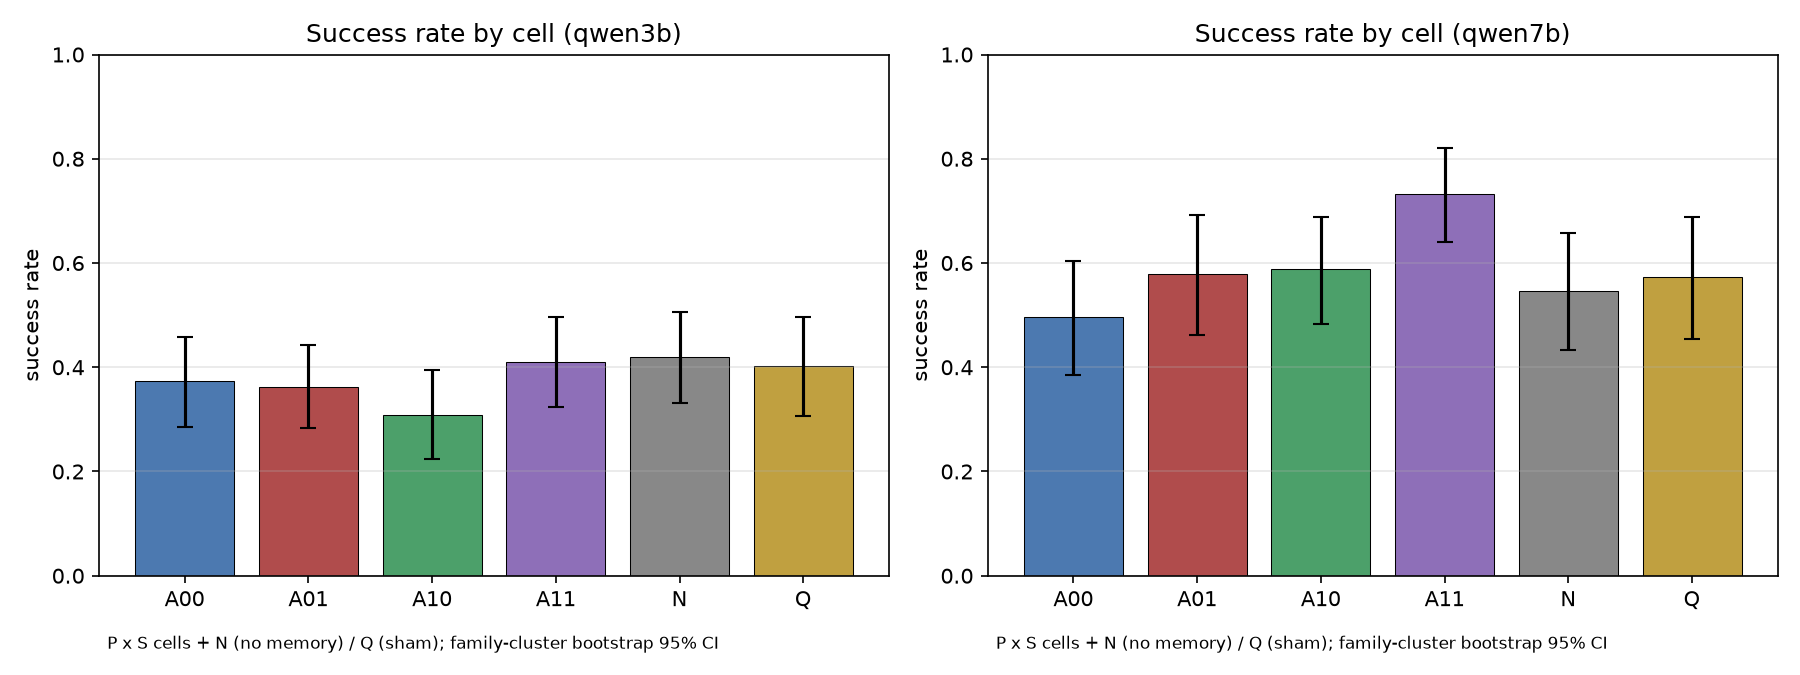
\includegraphics[width=\linewidth]{figs/fig1_cells_success.png}
  \caption{Stage-A cell success rates with 95\% family-cluster CIs. A11 (replay-like) dominates the 7B pooled gain; the 3B pattern differs---only A11 gets near-parity with N while A10 (clean structural) falls below the unrelated control, foreshadowing the scale reversal of Section~\ref{ssec:scale}.}
  \label{fig:fig1}
\end{figure}

\begin{figure}[t]
  \centering
  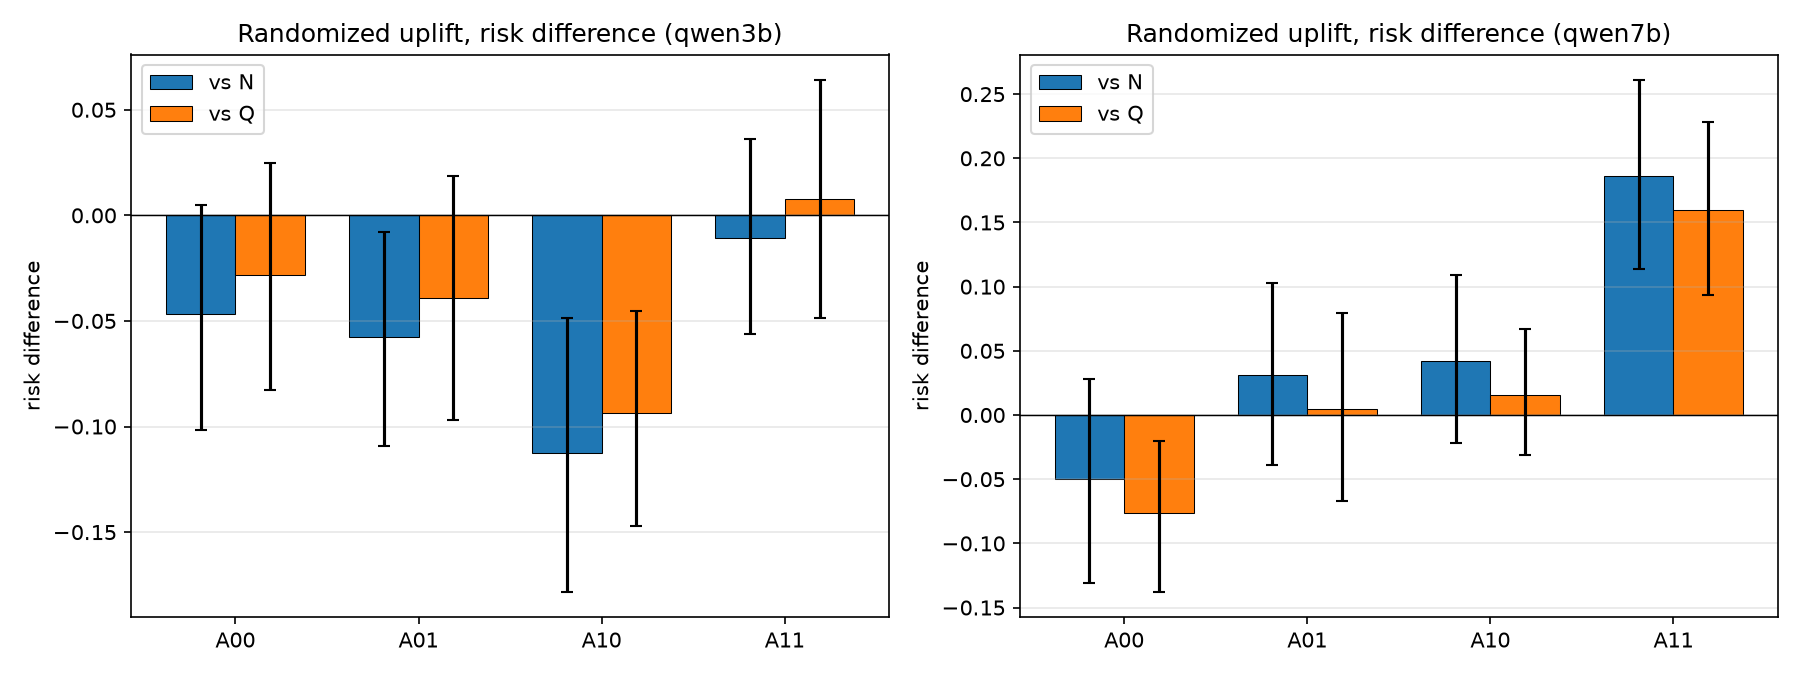
\includegraphics[width=\linewidth]{figs/fig2_uplift.png}
  \caption{Risk differences relative to N and Q. The format/context effect ($Q-N$) hugs zero; the decomposition separates a small structural term from a large replay term; 3B only benefits through A11.}
  \label{fig:fig2}
\end{figure}

\begin{figure}[t]
  \centering
  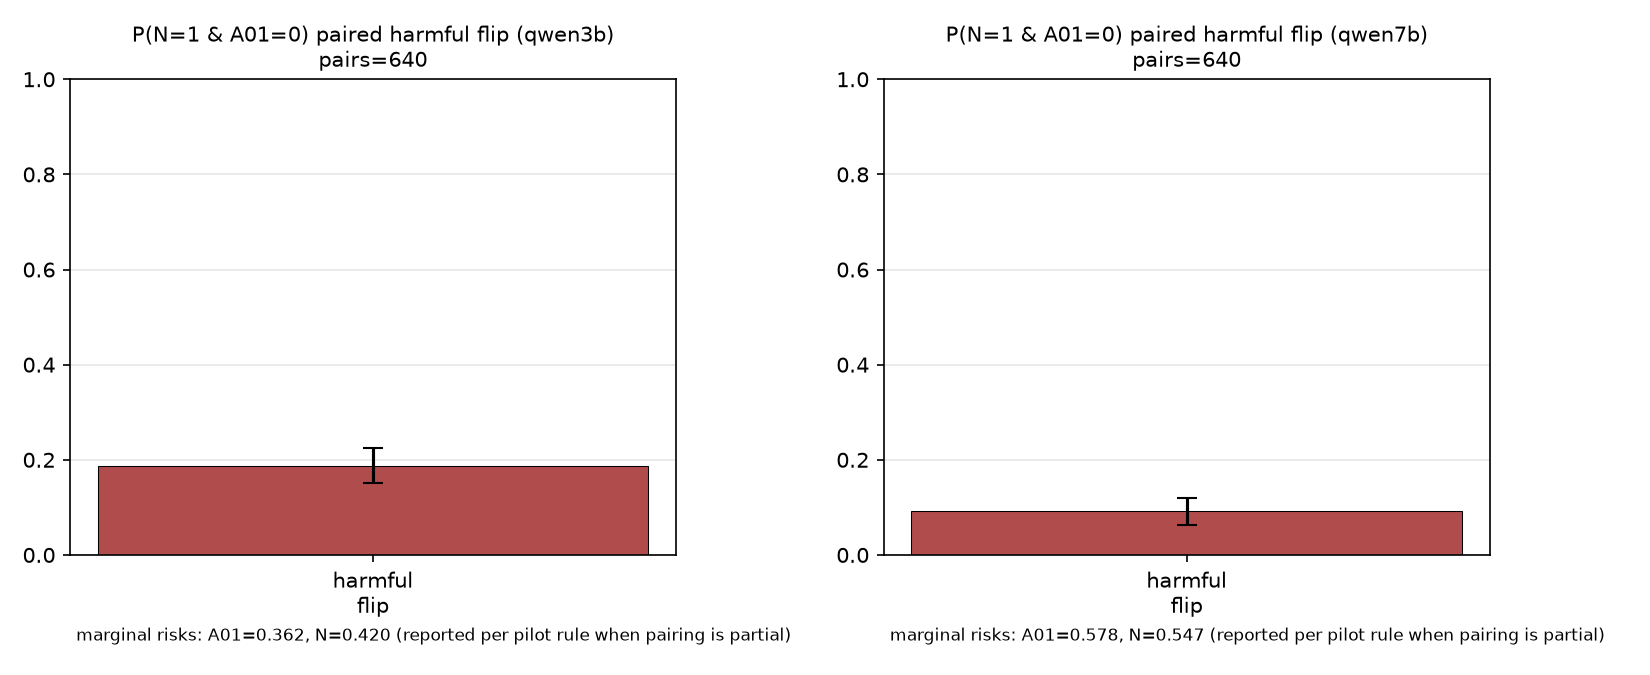
\includegraphics[width=\linewidth]{figs/fig4_harmful_flip.png}
  \caption{Paired harmful flips, A01 cell. Concentration on branches where the near-miss program semantically differs from the correct program, not a uniform effect; magnitude falls with scale.}
  \label{fig:fig4}
\end{figure}

\begin{figure}[t]
  \centering
  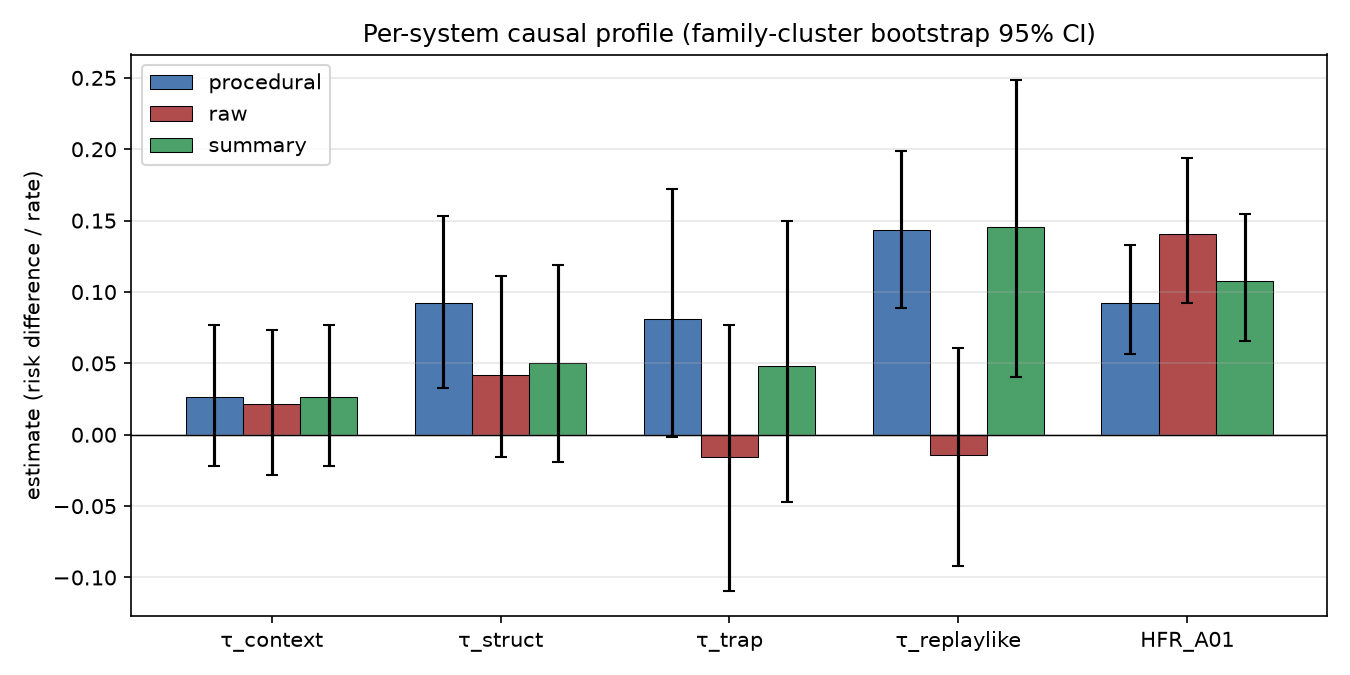
\includegraphics[width=\linewidth]{figs/hc_profiles.png}
  \caption{Form/coverage arms on fresh families (H3). Top pad: A10/A11 rates per arm; bottom pad: replay term per arm with 95\% CIs. Complete transcripts realize replay materially (TOST rejects $\pm3$pp equivalence), hard-truncated (eco) does not; form contrast is Holm-null in 8 tests.}
  \label{fig:h3}
\end{figure}

\begin{figure}[t]
  \centering
  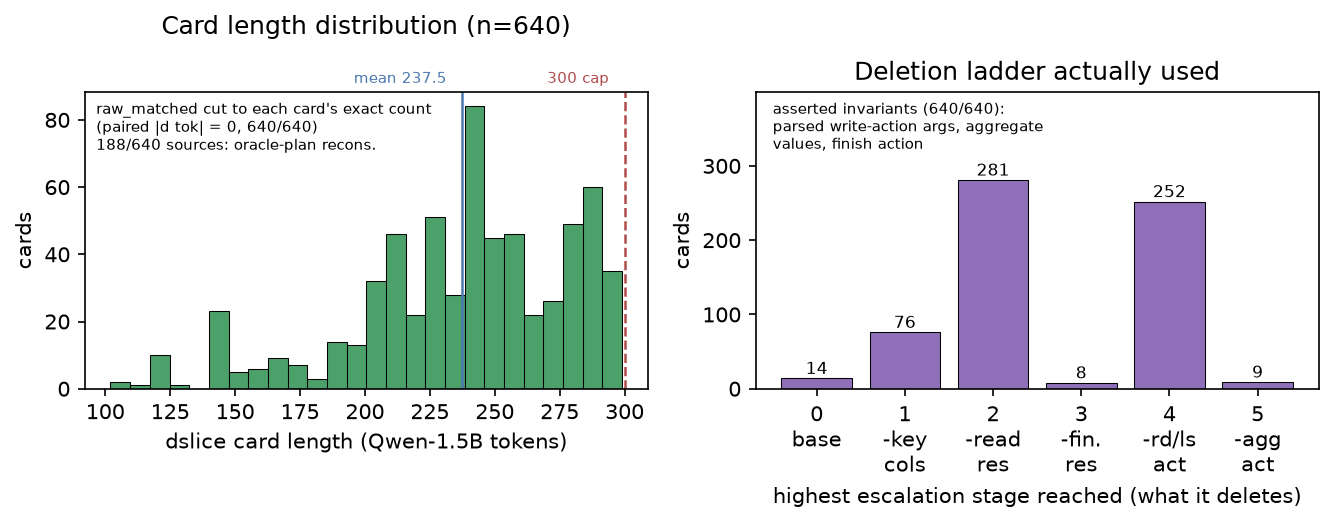
\includegraphics[width=0.92\linewidth]{figs/fig_hdc_cards.png}
  \caption{\textsc{dslice} card construction audit (Section~\ref{sec:deployment}). Left: realized card lengths (mean 237.5 tokens vs.\ the 300 cap); the paired \textsc{raw\_matched} control is cut to each card's exact count, so token budgets match per card by construction. 188/640 sources are oracle-plan reconstructions of failed harvests (provenance disclosure in \S\ref{ssec:dctest}); all arms share identical sources. Right: highest deletion stage reached per card (1: read-summary key columns; 2: read result lines; 3: finish \emph{result}; 4: non-decision action lines; 5: aggregate action lines). Asserted invariants---parsed write-action arguments, aggregate values, finish action---hold in 640/640 cards (0 QA failures).}
  \label{fig:hdccards}
\end{figure}

\begin{figure}[t]
  \centering
  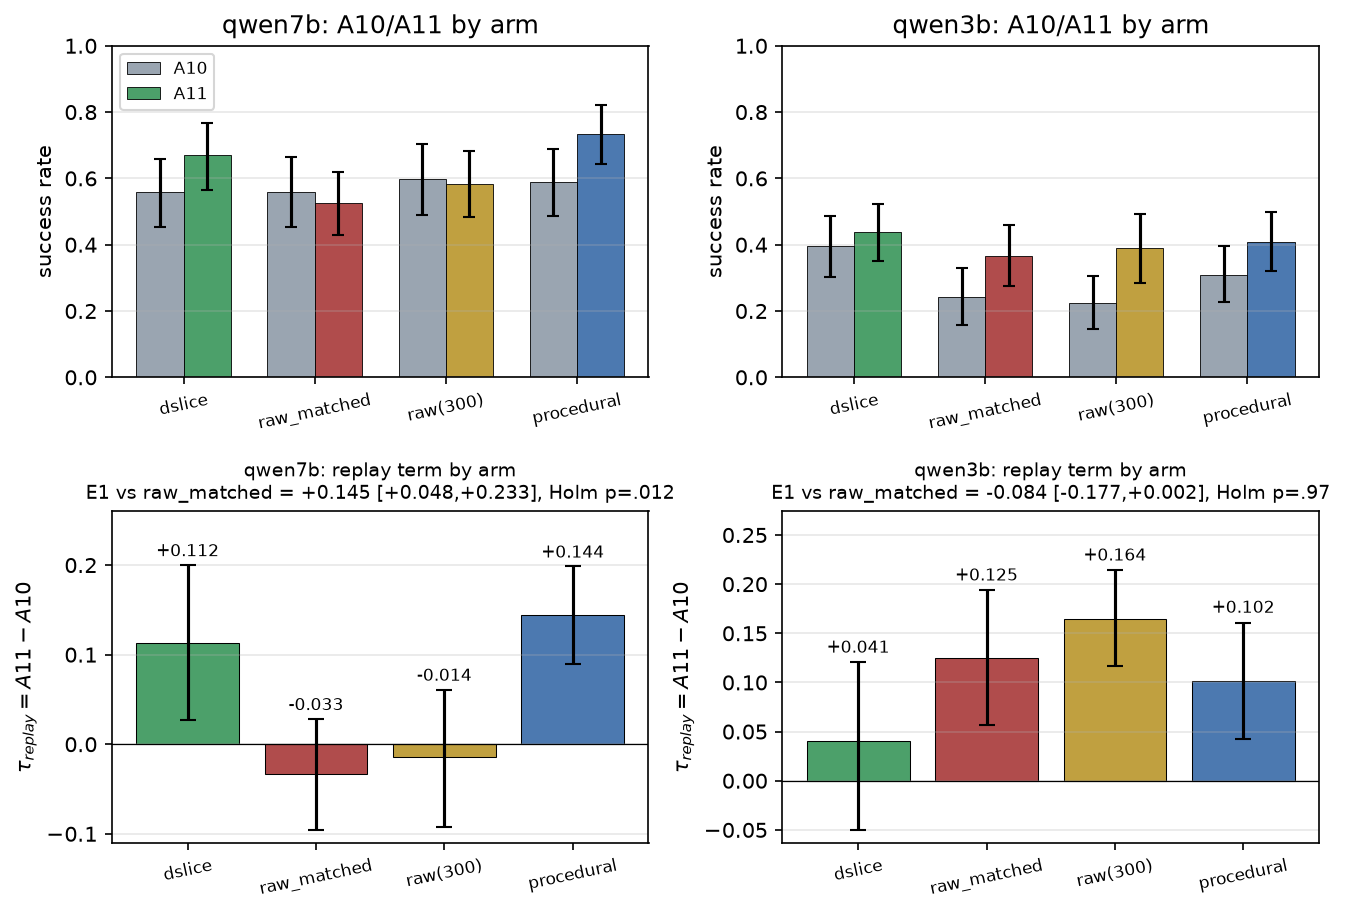
\includegraphics[width=\linewidth]{figs/fig_hdc_contrasts.png}
  \caption{Deployment result (Section~\ref{sec:deployment}). Top: A10/A11 rates per arm per model, family-cluster 95\% CIs. Bottom: replay term per arm. On the pooled 7B grid, \textsc{dslice} realizes replay while exactly-paired truncation realizes none (E1 $=+0.145$, Holm $p=.012$); at 3B there is no pooled evidence of benefit (E1 $-0.084$ [$-0.177$,$+0.002$], Holm $p=.97$). A post-hoc provenance stratification qualifies both: on authentic model-generated sources E1 $=+0.041$ [$-0.078$,$+0.149$] (7B) and $-0.226$ [$-0.347$,$-0.104$] (3B), and a direct interaction estimates oracle-minus-authentic E1 at $+0.382$ [$+0.166$,$+0.606$] (7B) and $+0.523$ [$+0.306$,$+0.783$] (3B); the pooled 7B win is carried by oracle-reconstructed sources (Appendix~\ref{app:hdc}).}
  \label{fig:hdc}
\end{figure}

\section{Discussion}

\subsection{What changes in the aggregate narrative}

Our three main numbers are uncomfortable reading for several widely-quoted results. The pooled matched-content effect that aggregate benchmarks report is replay-dominated here ($72\%$ from the A11 leg), but the same pooled statistic would have survived two very different decompositions---a trap (A01) moving 18.8\% of solvable tasks to failure for 3B, or a clean 9.2pp structural transfer for 7B. ``Memory helps'' is an aggregate claim that the community has been shipping where it wasn't measurable. System-level transplant experiments could not have caught this difference (\S\ref{sec:gatec}): their factors change systems, not the semantic relation between a candidate memory and a target task.

\subsection{Deployment reading}

Concrete, directly-usable implications:
\begin{enumerate}[leftmargin=1.8em]
  \item \textbf{Stop consulting aggregate accuracy} when comparing memory systems. Report the four numbers: context, clean structural, replay, and flip rate.
  \item \textbf{Preserve the decision+finish of an episode} in any stored form. Our truncation results show that a 300-token cap that silently eats the decision step turns useful experience into effectively zero-signal text ($\taureplay \approx 0$), even with perfect surface match.
  \item \textbf{Do not trust an LLM's own equivalence check} for memory admission. We tested retrieval-grade judgment plus intent-mismatch alarms; neither recovers the label at usable strength in our environment. Program-equivalence estimation is an inference problem, not a lookup.
  \item \textbf{Treat near-miss content as a fault channel}, not as style noise: paired harmful flips are model-scale-dependent (18.8\% at 3B, 9.2\% at 7B) and branch-conditional on program divergence.
  \item \textbf{Expect structural transfer to be capability-gated}, not universal: the structural term changed sign between 3B and 7B under identical content and budget. If your fleet includes small models, measure whether structural memory \emph{hurts} it before shipping.
\end{enumerate}

\subsection{Limitations}

\begin{enumerate}[leftmargin=1.8em]
  \item \textbf{Synthetic environment.} All identification is by construction in one SQLite world with programmatic predicates; transport to rich real tasks is checked only coarsely (a small ALFWorld external check; we do not claim AppWorld-scale external validity). The Tas test is whether aggregate directions repeat, not magnitudes.
  \item \textbf{Narrow model coverage.} Two frozen Qwen2.5 scales for inference; one family. A Llama-3.1-8B replication is in flight; sign conclusions could be family-specific and we will qualify them accordingly (Section~\ref{app:families}).
  \item \textbf{Equivalence-class ontologys.} Our partial-order classes are stricter than unconstrained "task similarity"; alternative operationalizations (e.g., embedding-based clustering of hidden workflows) are not evaluated and could reshuffle A10 vs A01 at the boundary.
  \item \textbf{Trap-plane surface readability.} Chip-level near-miss detection from text was possible at family hold-out (AUC 0.996); we register it as a semantics of benchmark traps rather than leakage, but it limits what "unreadable label" claims can be made on that axis.
  \item \textbf{Analysis breadth.} worry: power is limited by 40/32 family clusters; decompositions at archetype level, though reported, have wide intervals and are exploratory only.
\end{enumerate}

\subsection{What should come next}

The applied sequel is a transportable-memory admission rule validated the same way---we did not run it because it would be governed against standards we cannot yet meet (Section~\ref{sec:boundaries}). The theory sequel is a distributional-robustness treatment of transformation-shifted memory utility \citep{angelopoulos2024crc,wu2016conservative,jalaldoust2024transport}. And the measurement sequel asks how far these estimates agree with the observational estimators people can only compute without our oracle.


\bibliography{references}
\bibliographystyle{iclr2027_conference}

\appendix
\section{Reproducibility}
\label{app:repro}

All artifacts at \texttt{github.com/anonymous/CausalMemBench} upon de-anonymization:
\begin{itemize}[leftmargin=1.4em]
  \item generator \texttt{pilot/generate\_families.py} (pilot seed 20260807, H3 seed 20260809); sealed-vs-public split; oracle walker execution logs confirming 800/800 and 640/640 legal terminals;
  \item environment \texttt{pilot/env\_relationalops.py}, DSL \texttt{pilot/program\_dsl.py}, harness \texttt{pilot/harness.py} (vLLM 0.6.6.post1 / torch 2.5.1+cu124 on RTX A5000 24GB, fp16, temperature 0.7, top-p 0.9, max 12 steps $\times$ 512 tokens);
  \item rollouts JSONL: 16{,}896 rows with per-row commit, config-hash, model, versions, GPU;
  \item pre-registered protocols: GATE\_PROTOCOL Parts I--III dated 2026-08-07/08 before any analysis run;
  \item audit suite \texttt{pilot/audit/\{probes,difficulty\_robust,continuous\_s,equivalence\_audit\}.py}, blind annotations, judge outputs verbatim;
  \item analysis: family-cluster bootstrap utilities, Holm/TOST routines, and the exact \texttt{analyze.py/json} dumps reported here;
  \item design registers: RESEARCH\_LEDGER (pre-registration chain + external-review outcomes), §13 artifacts, construction rulings for H3 cards.
\end{itemize}

\section{Families and archetypes}
\label{app:families}

40 pilot families = 4 archetypes $\times$ 2 domains (crm/inv/ticket/cal) $\times$ 5 instances; 32 H3 families = 4/archetype $\times$ 8 schemas with disjoint parameters. For each family: 4 program-preserving siblings + 1 near-miss + a10 cross-domain partner + a00 unrelated partner, style counterbalanced by a 6-template Latin square, memories 200--300 Qwen-1.5B tokens measured by tokenizer, similarity buckets frozen against pilot distribution anchors.

\section{Deferred results (in-flight)}
\label{app:inflight}

Two replications were queued at submission time and are listed with their status for transparency:
\begin{itemize}[leftmargin=1.4em]
  \item \textbf{Llama-3.1-8B family-swap} on the identical 40-family grid (3840 rollouts): tests family-dependence of the structural-transfer sign flip (pending at commit time; analyze identically and report in camera-ready).
  \item \textbf{ALFWorld coarse external check} (3 families $\times$ 4 siblings $\times$ 4 cells $\times$ 3 seeds, Qwen2.5-7B): effect-ordering sanity in a non-synthetic environment (pending).
\end{itemize}
Neither is needed for the headline claims, which come only from the completed in-id data above.


\end{document}
